\documentclass[wide,a4paper,titlepage,12pt] {article}
\usepackage{polski}
\usepackage[UTF8]{inputenc}
\usepackage{listings}
\usepackage{slashbox}
\usepackage[table]{xcolor}
\usepackage{graphicx,pdflscape}
\usepackage{placeins}


\title{Grafika komputerowa}
\author{Jacek Wieczorek (181043)}

% Title page layout (fold)
\makeatletter
\renewcommand{\maketitle}{
\begin{titlepage}
  \begin{center}
    \vspace*{3cm}
    \LARGE \@title \par
    \vspace{2cm}
    \textit{\small Autor:}\par
    \normalsize \@author\par \normalsize
    \vspace{3cm}
    \textit{\small Prowadzący:}\par
    Dr inż. Tomasz Kapłon \par
    \vspace{2cm}
    Wydział Elektroniki\\ III rok\\ Pn TP 08.15 - 11.00\par
    \vspace{4cm}
    \small \@date
  \end{center}
\end{titlepage}
}
\makeatother
% Title page layout (end)



\begin{document}
\maketitle
  \section{Cel laboratorium}
  Ćwiczenie ma za zadanie pokazać, jak przy pomocy funkcji biblioteki OpenGL z rozszerzeniem GLUT można zrealizować prostą interakcję, polegającą na sterowaniu ruchem obiektu i położeniem obserwatora w przestrzeni 3-D. Do sterowania służyła będzie mysz. 
\section{Zad 1}
Celem pierwszego zadnia było wygenerowanie trójwymiarowego obrazu czajnika w rzucie perspektywicznym i zapewnienie możliwości jego skalowania i obracania za pomocą myszy : 
\begin{itemize}
	\item wciśnięty LPM i ruch w kierunku poziomym - obrót wokół osi $y$
	\item wciśnięty LPM i ruch w kierunku pionowym - obrót wokół osi $x$
	\item wciśnięty PPM i ruch w kierunku pionowym - zbliżenie (zoom)
\end{itemize} 
Funkcja odpowiedzialna za odczytywanie odpowiednich sekwencji myszy : 
\lstset{ %
    language=c++,                % choose the language of the code
    basicstyle=\scriptsize,       % the size of the fonts that are used for the code
    numbers=left,                   % where to put the line-numbers
    numberstyle=\scriptsize,      % the size of the fonts that are used for the line-numbers
    stepnumber=10,                   % the step between two line-numbers. If it's 1 each line 
                                    % will be numbered
    numbersep=9pt,                  % how far the line-numbers are from the code
    % backgroundcolor=\color{white},  % choose the background color. You must add \usepackage{color}
    showspaces=false,               % show spaces adding particular underscores
    showstringspaces=false,         % underline spaces within strings
    showtabs=false,                 % show tabs within strings adding particular underscores
    % frame=single,                 % adds a frame around the code
    % tabsize=2,                  % sets default tabsize to 2 spaces
    % captionpos=b,                   % sets the caption-position to bottom
    breaklines=true,                % sets automatic line breaking
    % breakatwhitespace=false,        % sets if automatic breaks should only happen at whitespace
    % title=\lstname,                 % show the filename of files included with \lstinputlisting;
                                    % also try caption instead of title
    % escapeinside={\%*}{*)},         % if you want to add a comment within your code
    % morekeywords={*,...}            % if you want to add more keywords to the set
    }
    \lstinputlisting{czajnikMouse.cpp}
\newpage\noindent
Funkcja odpowiedzialna za wyznaczanie o ile ma nastapić obrót lub zoom 
\lstset{ %
    language=c++,                % choose the language of the code
    basicstyle=\scriptsize,       % the size of the fonts that are used for the code
    numbers=left,                   % where to put the line-numbers
    numberstyle=\scriptsize,      % the size of the fonts that are used for the line-numbers
    stepnumber=10,                   % the step between two line-numbers. If it's 1 each line 
                                    % will be numbered
    numbersep=9pt,                  % how far the line-numbers are from the code
    % backgroundcolor=\color{white},  % choose the background color. You must add \usepackage{color}
    showspaces=false,               % show spaces adding particular underscores
    showstringspaces=false,         % underline spaces within strings
    showtabs=false,                 % show tabs within strings adding particular underscores
    % frame=single,                 % adds a frame around the code
    % tabsize=2,                  % sets default tabsize to 2 spaces
    % captionpos=b,                   % sets the caption-position to bottom
    breaklines=true,                % sets automatic line breaking
    % breakatwhitespace=false,        % sets if automatic breaks should only happen at whitespace
    % title=\lstname,                 % show the filename of files included with \lstinputlisting;
                                    % also try caption instead of title
    % escapeinside={\%*}{*)},         % if you want to add a comment within your code
    % morekeywords={*,...}            % if you want to add more keywords to the set
    }
    \lstinputlisting{czajnikSterowanie.cpp} 
\noindent
Funkcja odpowiedzialna za renderowanie widoku : 
\lstset{ %
    language=c++,                % choose the language of the code
    basicstyle=\scriptsize,       % the size of the fonts that are used for the code
    numbers=left,                   % where to put the line-numbers
    numberstyle=\scriptsize,      % the size of the fonts that are used for the line-numbers
    stepnumber=10,                   % the step between two line-numbers. If it's 1 each line 
                                    % will be numbered
    numbersep=9pt,                  % how far the line-numbers are from the code
    % backgroundcolor=\color{white},  % choose the background color. You must add \usepackage{color}
    showspaces=false,               % show spaces adding particular underscores
    showstringspaces=false,         % underline spaces within strings
    showtabs=false,                 % show tabs within strings adding particular underscores
    % frame=single,                 % adds a frame around the code
    % tabsize=2,                  % sets default tabsize to 2 spaces
    % captionpos=b,                   % sets the caption-position to bottom
    breaklines=true,                % sets automatic line breaking
    % breakatwhitespace=false,        % sets if automatic breaks should only happen at whitespace
    % title=\lstname,                 % show the filename of files included with \lstinputlisting;
                                    % also try caption instead of title
    % escapeinside={\%*}{*)},         % if you want to add a comment within your code
    % morekeywords={*,...}            % if you want to add more keywords to the set
    }
    \lstinputlisting{czajnikRenderScene.cpp}

W celu zastosowania rzutu perspektywicznego, w funkcji $ChangeSize$ zamiast funkcji $glOrtho()$ skorzystaliśmy z funkcji $gluPerspective()$.

\begin{figure}[htbp]
	 		\begin{center}
         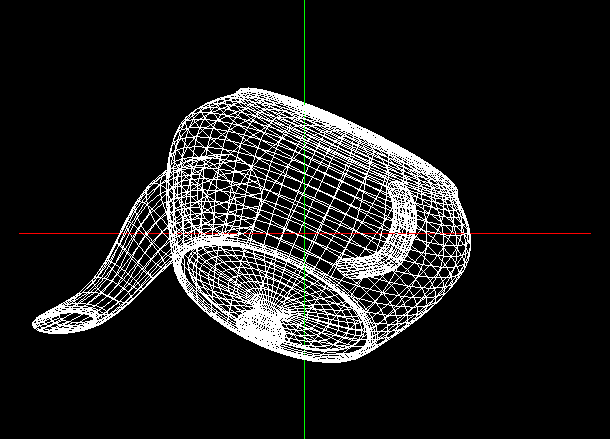
\includegraphics[scale=0.6]{cz3.PNG}
      \caption{Czajnik}
     \end{center}
  \end{figure}
\begin{figure}[htbp]
	 		\begin{center}
         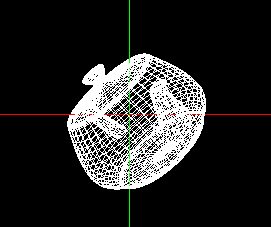
\includegraphics[scale=0.6]{cz2.PNG}
      \caption{Czajnik - zoom}
     \end{center}
  \end{figure}
\newpage
\section{Zad 2}
\paragraph{}
Drugie zadanie polegało na możliwości "sterowania" jajkiem z laboratorium 3 za pomocą zmiany punktu widzenia, przy następujących założeniach:
\begin{itemize}
	\item Jajko znajduje się w środku układu współrzędnych
	\item Punkt obserwatora może się poruszać po po powierzchni sfery o promieniu $R$ i środku będącym środkiem ukłądu współrzędnych
	\item Sterowanie odbywać się będzie za pomocą dwóch kątów : kąt azymutu - $\Theta$ o kąt elewacji - $\Phi$
\end{itemize}

\begin{figure}[htbp]
	\begin{center}
        	 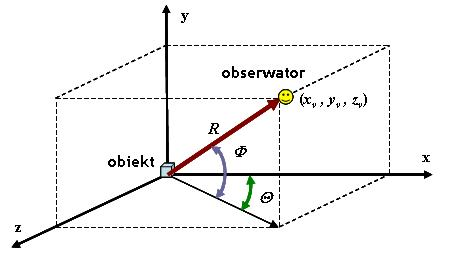
\includegraphics[scale=1]{ukl.jpg}
     	 \caption{Układ, obiekt, obserwator i kąty azymutu i elewacji}
   	  \end{center}
\end{figure}
Zależności wiążące współrzędne punktu obserwatora z promieneim sfery i kątami:
\begin{figure}[htbp]
	\begin{center}
        	 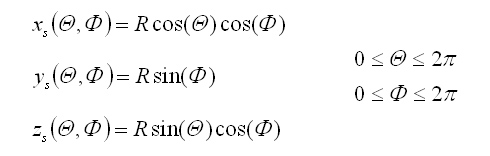
\includegraphics[scale=0.65]{zal.jpg}

   	  \end{center}
\end{figure}
\newpage
Założenia sterowania:
\begin{itemize}
	\item Przy wciśniętym LPM i ruch w kierunku poziomym zmianie ulega kąt azymutu
	\item Przy wciśniętym LPM i ruch w kierunku pionowym zmianie ulega kąt elewacji
	\item Przy wciśniętym PPM i ruchu w kierunku pionowym ulega zmianie $R$
\end{itemize}
Funkcja odpowiedzialna za renderowanie widoku : 
\lstset{ %
    language=c++,                % choose the language of the code
    basicstyle=\scriptsize,       % the size of the fonts that are used for the code
    numbers=left,                   % where to put the line-numbers
    numberstyle=\scriptsize,      % the size of the fonts that are used for the line-numbers
    stepnumber=10,                   % the step between two line-numbers. If it's 1 each line 
                                    % will be numbered
    numbersep=9pt,                  % how far the line-numbers are from the code
    % backgroundcolor=\color{white},  % choose the background color. You must add \usepackage{color}
    showspaces=false,               % show spaces adding particular underscores
    showstringspaces=false,         % underline spaces within strings
    showtabs=false,                 % show tabs within strings adding particular underscores
    % frame=single,                 % adds a frame around the code
    % tabsize=2,                  % sets default tabsize to 2 spaces
    % captionpos=b,                   % sets the caption-position to bottom
    breaklines=true,                % sets automatic line breaking
    % breakatwhitespace=false,        % sets if automatic breaks should only happen at whitespace
    % title=\lstname,                 % show the filename of files included with \lstinputlisting;
                                    % also try caption instead of title
    % escapeinside={\%*}{*)},         % if you want to add a comment within your code
    % morekeywords={*,...}            % if you want to add more keywords to the set
    }
    \lstinputlisting{jajkoRenderScene.cpp}
\paragraph{}
 W celu określenia położenia obserwatora wykorzystujemy funkcję $gluLoolAt()$. Trójelementowa tablica $viewer$ określa nam współrzędne $x,y,z$ obserwatora wyliczone za pomocą powyższych wzorów. Następne 3 parametry funkcji określają położenie środka układu współrzędnych, a ostatnie 3 kierunki wektorów. Ze względu na okresowość funkcji sinus i problem z pelnym obrotem jajka z powodu wartości zmiennej $y$, w określaniu kierunku wektora $Y$ skorzystaliśmy z parmetru $p$, który przyjmuje odpowiednio wartości $1$ i $-1$. W tym celu sprawdzamy czy kąt $\Phi$ nie przekracza wartości $\Pi$ lub $-\Pi$, jeżeli tak to dodajemy lub odejmujemy od niego równowarość $2*\Pi$, i w zalezności od wartości kąta $\Phi$ ustalamy odpowiednią wartość parametru $p$.
\paragraph{}
Pozostałe funkcje strujące są takie same jak w zadaniu poprzednim. W zadaniu wykorzystane zostało jajko z laboratorium nr 3.
\begin{figure}[htbp]
	\begin{center}
        	 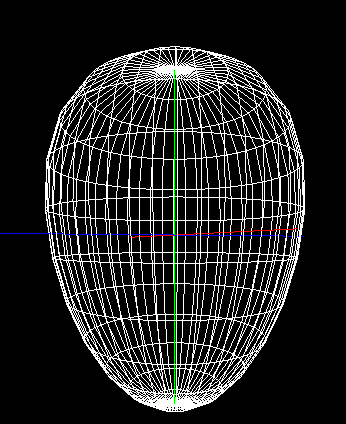
\includegraphics[scale=1]{j1.PNG}
	\caption{Jajko "do góry nogami"}
   	  \end{center}
\end{figure}
\begin{figure}[htbp]
	\begin{center}
        	 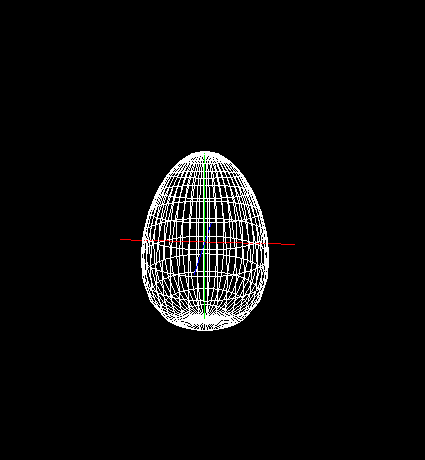
\includegraphics[scale=0.7]{j2.PNG}
	\caption{Jajko ze zmienjszonym promieniem $R$}
   	  \end{center}
\end{figure}
\begin{figure}[htbp]
	\begin{center}
        	 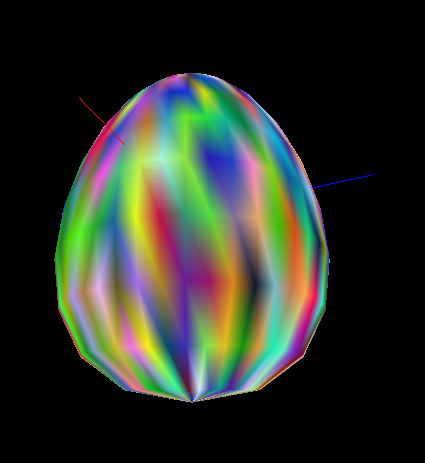
\includegraphics[scale=0.7]{j3.PNG}
	\caption{Jajko zbudowane z trójkątów}
   	  \end{center}
\end{figure}
\newpage
\section{Wnioski}
\paragraph{}
Interakcja obiektów w przestrzeni $3D$ z użytkownikiem z wykorzystaniem biblioteki $OpenGL$ i $GLUT$ nie jest tak skomplikowanym zadaniem. Probelemem okazały się matematyczne opisy równań, a zwłaszcza wyeliminowanie błędu obrotu jajka wynikającego z okresowości funckji sinus. Sama obsługa zdarzeń pochodzących od klawiatury, czy też myszy jest prosta i intuicyjna.
\end{document}